\clearpage
\item \points{40} {\bf Linear Classifiers (logistic regression and GDA)}

In this problem, we cover two probabilistic linear classifiers we have
covered in class so far. First, a discriminative linear classifier: logistic
regression. Second, a generative linear classifier: Gaussian discriminant
analysis (GDA). Both the algorithms find a linear decision boundary that
separates the data into two classes, but make different assumptions. Our goal
in this problem is to get a deeper understanding of the similarities and
differences (and, strengths and weaknesses) of these two algorithms.

For this problem, we will consider two datasets, provided in the following
files:
\begin{enumerate}[label=\roman*.]
	\item \url{data/ds1_{train,valid}.csv}
	\item \url{data/ds2_{train,valid}.csv}
\end{enumerate}
Each file contains $m$ examples, one example $(x^{(i)}, y^{(i)})$ per row.
In particular, the $i$-th row contains columns $x^{(i)}_0\in\Re$,
$x^{(i)}_1\in\Re$, and $y^{(i)}\in\{0, 1\}$. In the subproblems that follow, we
will investigate using logistic regression and Gaussian discriminant analysis
(GDA) to perform binary classification on these two datasets.

\begin{enumerate}
	\item \subquestionpoints{10}
In lecture we saw the average empirical loss for logistic regression:
\begin{equation*}
	J(\theta)
	= -\frac{1}{m} \sum_{i=1}^m y^{(i)}\log(h_{\theta}(x^{(i)}))
		+  (1 - y^{(i)})\log(1 - h_{\theta}(x^{(i)})),
\end{equation*}
where $y^{(i)} \in \{0, 1\}$, $h_\theta(x) = g(\theta^T x)$ and
$g(z) = 1 / (1 + e^{-z})$.

Find the Hessian $H$ of this function, and show that for any vector $z$, it
holds true that
%
\begin{equation*}
    z^T H z \ge 0.
\end{equation*}
%
{\bf Hint:} You may want to start by showing that
$\sum_i\sum_j z_i x_i x_j z_j = (x^Tz)^2 \geq 0$. Recall also that
$g'(z) = g(z)(1-g(z))$.

{\bf Remark:} This is one of the standard ways of showing that the matrix $H$
is positive semi-definite, written ``$H \succeq 0$.''  This implies that $J$ is
convex, and has no local minima other than the global one. If you have some
other way of showing $H \succeq 0$, you're also welcome to use your method
instead of the one above.

\ifnum\solutions=1 {
  \begin{answer}

The hessian derivation
Take the derivative w.r.t. $\theta_j$,  $h'(x) = g'(\theta^T x) = g(\theta^T x)(1-g(\theta^T x) x_j$ for the jth component.
\begin{eqnarray*}
    \frac{\partial J}{\partial \theta_j}
	&=& -\frac{1}{m} \sum_{i=1}^m \left(y^{(i)} \frac{h_{\theta}(x^{(i)}) (1-h_{\theta}(x^{(i)})} {h_{\theta}(x^{(i)}} x_j
	+ (1 - y^{(i)}) \frac{-h_{\theta}(x^{(i)})  (1-h_{\theta}(x^{(i)}) } {h_{\theta}(x^{(i)}} x_j \right) \\
	&=& -\frac{1}{m} \sum_{i=1}^m \left(y^{(i)}  (1-h_{\theta}(x^{(i)}) x_j
	- (1 - y^{(i)}) h_{\theta}(x^{(i)}) x_j \right) \\
	&=& -\frac{1}{m} \sum_{i=1}^m (y^{(i)} - h_{\theta}(x^{(i)})) x_j
\end{eqnarray*}

The Hessian is just the second order derivative of the cost. Observe the above $\frac{\partial J}{\partial \theta_j}$, 
only the $ h_{\theta}(x^{(i)}) x_j$ part is relevant.
\begin{eqnarray*}
    \frac{\partial^2 J}{\partial \theta_j \theta_k}
	&=& \frac{1}{m} \sum_{i=1}^m  h_{\theta}(x^{(i)})(1 -  h_{\theta}(x^{(i)})) x_j x_k \\
	&=& H_{jk}
\end{eqnarray*}
The diagonals where $j = k$ are also generalized by $H_{jk}$.

Proof of Hessian's PSD.

For any vector $z$, and any given sample $x^{(i)}$, 
consider only $H^{(i)}_{jk}=h_{\theta}(x^{(i)})(1 -  h_{\theta}(x^{(i)})) x_j x_k$:
\begin{eqnarray*}
z^T H^{(i)} z 
	&=& h_{\theta}(x^{(i)})(1 -  h_{\theta}(x^{(i)})) \sum_{j=1}^n \sum_{k=1}^n z_j x_j x_k z_k \\
	&=& h_{\theta}(x^{(i)})(1 -  h_{\theta}(x^{(i)})) (z^T x)^2 \\
	&\ge& 0
\end{eqnarray*}
The last step is true because the sigmoid function can only be (0,1). So $H^{(i)}$ is PSD.

The Hessian H is just the mean of all  $H^{(i)}$, so it is still a Hessian. 

Proved.

\end{answer}

} \fi

	\clearpage
\item \subquestionpoints{5} \textbf{Coding problem.}
Follow the instructions in \texttt{src/p01b\_logreg.py} to train a
logistic regression classifier using Newton's Method.
Starting with $\theta = \vec{0}$, run Newton's Method until the updates to
$\theta$ are small: Specifically,  train until the first iteration $k$ such
that $\|\theta_{k} - \theta_{k-1}\|_1 < \epsilon$, where
$\epsilon = 1\times 10^{-5}$. Make sure to write your model's predictions to
the file specified in the code.

\ifnum\solutions=1 {
  \begin{answer}
\end{answer}

} \fi

	\clearpage
\item \subquestionpoints{5}
Recall that in GDA we model the joint distribution of $(x, y)$ by the following
equations:
%
\begin{eqnarray*}
	p(y) &=& \begin{cases}
	\phi & \mbox{if~} y = 1 \\
	1 - \phi & \mbox{if~} y = 0 \end{cases} \\
	p(x | y=0) &=& \frac{1}{(2\pi)^{n/2} |\Sigma|^{1/2}}
		\exp\left(-\frac{1}{2}(x-\mu_{0})^T \Sigma^{-1} (x-\mu_{0})\right) \\
	p(x | y=1) &=& \frac{1}{(2\pi)^{n/2} |\Sigma|^{1/2}}
		\exp\left(-\frac{1}{2}(x-\mu_1)^T \Sigma^{-1} (x-\mu_1) \right),
\end{eqnarray*}
%
where $\phi$, $\mu_0$, $\mu_1$, and $\Sigma$ are the parameters of our model.

Suppose we have already fit $\phi$, $\mu_0$, $\mu_1$, and $\Sigma$, and now
want to predict $y$ given a new point $x$. To show that GDA results in a
classifier that has a linear decision boundary, show the posterior distribution
can be written as
%
\begin{equation*}
	p(y = 1\mid x; \phi, \mu_0, \mu_1, \Sigma)
	= \frac{1}{1 + \exp(-(\theta^T x + \theta_0))},
\end{equation*}
%
where $\theta\in\Re^n$ and $\theta_{0}\in\Re$ are appropriate functions of
$\phi$, $\Sigma$, $\mu_0$, and $\mu_1$.

\ifnum\solutions=1{
  \begin{answer}

Derive the posterior distribution from GDA model:

\begin{eqnarray*}
	p(y = 1\mid x)
	&=& \frac{p(x \mid y = 1) p(y = 1)}{p(x \mid y = 0) p(y = 0) + p(x \mid y = 1) p(y = 1)} \\
	&=& \frac {\frac{1}{(2\pi)^{n/2} |\Sigma|^{1/2}} exp \left( -\frac{1}{2}(x-\mu_1)^T \Sigma^{-1}(x-\mu_1)\right) \phi}
		{\frac{1}{(2\pi)^{n/2} |\Sigma|^{1/2}} \left[ exp \left( -\frac{1}{2}(x-\mu_1)^T \Sigma^{-1}(x-\mu_1)\right) \phi
		+ exp \left( -\frac{1}{2}(x-\mu_0)^T \Sigma^{-1}(x-\mu_0)\right) (1-\phi) \right ]} \\
	&=& \frac { \phi exp \left( -\frac{1}{2}(x-\mu_1)^T \Sigma^{-1}(x-\mu_1)\right)}
		{ \phi exp \left( -\frac{1}{2}(x-\mu_1)^T \Sigma^{-1}(x-\mu_1)\right)
		+ (1-\phi) exp \left( -\frac{1}{2}(x-\mu_0)^T \Sigma^{-1}(x-\mu_0)\right)} \\
	&=& \frac {1} {1 + \frac{1-\phi}{\phi} \exp \left (\frac{1}{2}(x-\mu_1)^T \Sigma^{-1}(x-\mu_1) 
		- \frac{1}{2}(x-\mu_0)^T \Sigma^{-1}(x-\mu_0) \right)} \\
	&=& \frac {1} {1 + exp \left( (\mu_0 - \mu_1)^T \Sigma^{-1} x 
		- \frac{1}{2}(\mu_0^T \Sigma^{-1}\mu_0 - \mu_1^T \Sigma^{-1}\mu_1)
		+ log (\frac{1-\phi}{\phi}) \right)}
\end{eqnarray*}

Set parameters $\theta$ and $\theta_0$ and rewrite the posterior:
\begin{eqnarray*}
	\theta &=& \mu_0 - \mu_1)^T \Sigma^{-1} \\
	\theta_0 &=& \frac{1}{2}(\mu_0^T \Sigma^{-1}\mu_0 - \mu_1^T \Sigma^{-1}\mu_1)	+ log (\frac{1-\phi}{\phi}) \\
	p(y = 1\mid x; \phi, \mu_0, \mu_1, \Sigma)
	&=& \frac{1}{1 + \exp(-(\theta^T x + \theta_0))}
\end{eqnarray*}
Q.E.D.
\end{answer}

}\fi

	\clearpage
\item \subquestionpoints{7} For this part of the problem only, you may
  assume $n$ (the dimension of $x$) is 1, so that $\Sigma = [\sigma^2]$ is
  just a real number, and likewise the determinant of $\Sigma$ is given by
  $|\Sigma| = \sigma^2$.  Given the dataset, we claim that the maximum
  likelihood estimates of the parameters are given by
  \begin{eqnarray*}
    \phi &=& \frac{1}{m} \sum_{i=1}^m 1\{y^{(i)} = 1\} \\
\mu_{0} &=& \frac{\sum_{i=1}^m 1\{y^{(i)} = {0}\} x^{(i)}}{\sum_{i=1}^m
1\{y^{(i)} = {0}\}} \\
\mu_1 &=& \frac{\sum_{i=1}^m 1\{y^{(i)} = 1\} x^{(i)}}{\sum_{i=1}^m 1\{y^{(i)}
= 1\}} \\
\Sigma &=& \frac{1}{m} \sum_{i=1}^m (x^{(i)} - \mu_{y^{(i)}}) (x^{(i)} -
\mu_{y^{(i)}})^T
  \end{eqnarray*}
  The log-likelihood of the data is
  \begin{eqnarray*}
\ell(\phi, \mu_{0}, \mu_1, \Sigma) &=& \log \prod_{i=1}^m p(x^{(i)} , y^{(i)};
\phi, \mu_{0}, \mu_1, \Sigma) \\
&=& \log \prod_{i=1}^m p(x^{(i)} | y^{(i)}; \mu_{0}, \mu_1, \Sigma) p(y^{(i)};
\phi).
  \end{eqnarray*}
By maximizing $\ell$ with respect to the four parameters,
prove that the maximum likelihood estimates of $\phi$, $\mu_{0}, \mu_1$, and
$\Sigma$ are indeed as given in the formulas above.  (You may assume that there
is at least one positive and one negative example, so that the denominators in
the definitions of $\mu_{0}$ and $\mu_1$ above are non-zero.)

\ifnum\solutions=1 {
  \begin{answer}

The bernoulli pdf can be written as $p(y) = \phi^y (1-\phi)^{(1-y)}$, hence:
\begin{eqnarray*}
\ell(\phi, \mu_{0}, \mu_1, \Sigma) 
	&=& \sum_{i=1}^m \log \phi^{y^{(i)}} (1-\phi)^{(1-y^{(i)})} \\
	&+& \sum_{i=1,y^{(i)}=1}^m \left( -\frac{1}{2}(x^{(i)}-\mu_1)^T \Sigma^{-1} (x^{(i)}-\mu_1) + \log {\frac{1}{(2\pi)^{n/2} |\Sigma|^{1/2}} }\right )\\
	&+& \sum_{i=1,y^{(i)}=0}^m \left( -\frac{1}{2}(x^{(i)}-\mu_0)^T \Sigma^{-1} (x^{(i)}-\mu_0) + \log {\frac{1}{(2\pi)^{n/2} |\Sigma|^{1/2}} }\right )\\
	&=& \sum_{i=1}^m y^{(i)} \log \phi + \sum_{i=1}^m (1-y^{(i)}) \log (1-\phi) \\
\end{eqnarray*}

Gradient w.r.t. parameter $\phi$:
\begin{eqnarray*}
\frac{\partial \ell}{\partial \phi}
	&=& \frac{\partial}{\partial \phi} \left (\sum_{i=1}^m y^{(i)} \log \phi + \sum_{i=1}^m (1-y^{(i)}) \log (1-\phi) \right)\\
	&=& \frac{\sum_{i=1}^m y^{(i)}}{\log \phi} - \frac{\sum_{i=1}^m (1-y^{(i)})}{\log (1-\phi)} \\
\end{eqnarray*}
Set it to 0 vector:
\begin{eqnarray*}
	\frac{\sum_{i=1}^m y^{(i)}}{\log \phi} = \frac{m- \sum_{i=1}^m y^{(i)}} {\log (1-\phi)} \\
	\Rightarrow \phi = \frac{1}{m} \sum_{i=1}^m 1\{y^{(i)} = 1\}
\end{eqnarray*}

Gradient w.r.t. parameter $\mu_1$, the same to $\mu_0$:
\begin{eqnarray*}
\frac{\partial \ell}{\partial \mu_1}
	&=& \frac{\partial}{\partial \mu_1} \sum_{i=1,y^{(i)}=1}^m \left( -\frac{1}{2}(x^{(i)}-\mu_1)^T \Sigma^{-1} (x^{(i)}-\mu_1) 
		+ \log {\frac{1}{(2\pi)^{n/2} |\Sigma|^{1/2}} }\right ) \\
	&=& -\sum_{i=1}^m 1\{y^{(i)}=1\}(x^{(i)}-\mu_1)^T \Sigma^{-1} \\
\end{eqnarray*}
The derivative w.r.t. $\mu_0$ is the same. Set these to 0 vector and get:
\begin{eqnarray*}
	\mu_0 = \frac{\sum_{i=1}^m 1\{y^{(i)} = 0\} x^{(i)}}{\sum_{i=1}^m 1\{y^{(i)} = 0\}} \\
	\mu_1 = \frac{\sum_{i=1}^m 1\{y^{(i)} = 1\} x^{(i)}}{\sum_{i=1}^m 1\{y^{(i)} = 1\}}
\end{eqnarray*}

For the gradient w.r.t. the covariance matrix $\Sigma$, it is still a nxn matrix; 
it has the similar steps of math work. Here we can use $\mu_{y^{(i)}}$ for both 0 and 1 classes. 
\begin{eqnarray*}
\frac{\partial \ell}{\partial \Sigma}
	&=& \frac{\partial}{\partial \Sigma} \sum_{i=1}^m \left( -\frac{1}{2}(x^{(i)}-\mu_{y^{(i)}})^T \Sigma^{-1} (x^{(i)}-\mu_{y^{(i)}}) 
		+ \log {\frac{1}{(2\pi)^{n/2} |\Sigma|^{1/2}} }\right ) \\
	&=& -\frac{\partial}{\partial \Sigma} \sum_{i=1}^m \left( \frac{1}{2}(x^{(i)}-\mu_{y^{(i)}})^T \Sigma^{-1} (x^{(i)}-\mu_{y^{(i)}}) 
		+ \frac{1}{2} \log {|\Sigma|}\right ) \\
	&=& \frac{1}{2} \left (\sum_{i=1}^m (x^{(i)}-\mu_{y^{(i)}})(x^{(i)}-\mu_{y^{(i)}})^T\Sigma^{-2} - m \Sigma^{-1} \right )
\end{eqnarray*}

Again set it to 0 matrix and right multiply by $\Sigma^2$, get $\Sigma$:
\begin{eqnarray*}
\Sigma &=& \frac{1}{m} \sum_{i=1}^m (x^{(i)} - \mu_{y^{(i)}}) (x^{(i)} - \mu_{y^{(i)}})^T
\end{eqnarray*}

\end{answer}

} \fi

	\clearpage
\item \subquestionpoints{3} \textbf{Coding problem.}
In \texttt{src/p01e\_gda.py}, fill in the code to
calculate $\phi$, $\mu_{0}$, $\mu_{1}$, and $\Sigma$, use these parameters
to derive $\theta$, and use the resulting GDA model to make predictions on the
validation set.

\ifnum\solutions=1 {
  \begin{answer}
\end{answer}

} \fi

	\clearpage
\item \subquestionpoints{5}
For Dataset 1, create a plot of the validation set with $x_1$ on the horizontal
axis, and $x_2$ on the vertical axis. To visualize the two classes, use a
different symbol for examples $x^{(i)}$ with $y^{(i)} = 0$ than for those with
$y^{(i)} = 1$. On the same figure, plot the decision boundary found by logistic
regression in part (b). Make an identical plot with the decision boundary found
by GDA in part (e).

\ifnum\solutions=1 {
\begin{answer}

\begin{figure}[h]
    \centering
    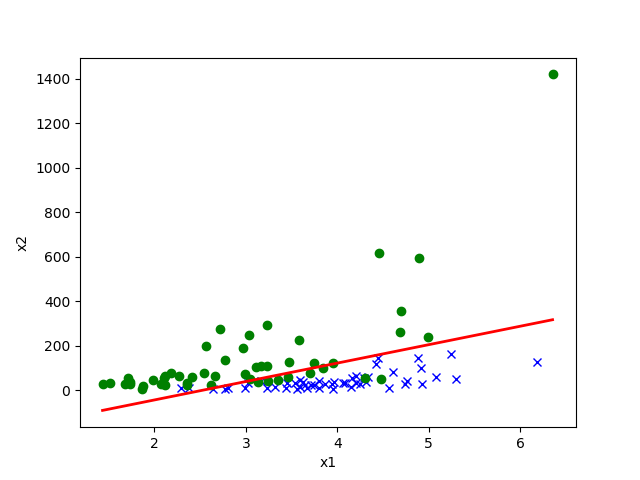
\includegraphics[width=0.6\textwidth]{p01b_pred_1_txt_lr_valid}
    \caption{Logistic Regression on Dataset 1}
\end{figure}

\begin{figure}[h]
    \centering
    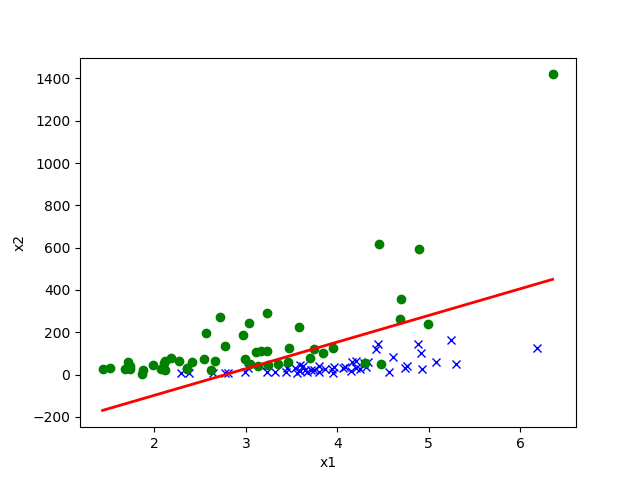
\includegraphics[width=0.6\textwidth]{p01e_pred_1_txt_gda_valid}
    \caption{GDA on Dataset 1}
\end{figure}
\end{answer}

} \fi

	\clearpage
\item \subquestionpoints{5}
Repeat the steps in part (f) for Dataset 2. On which dataset does GDA seem to
perform worse than logistic regression? Why might this be the case?

\ifnum\solutions=1{
  \begin{answer}

    \begin{figure}[h]
        \centering
        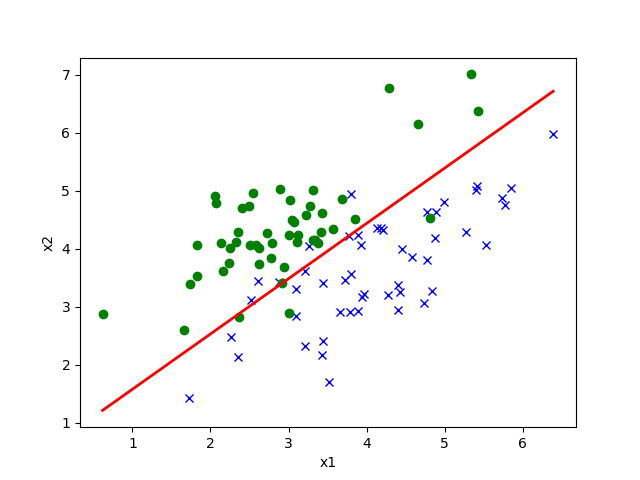
\includegraphics[width=0.6\textwidth]{p01b_pred_2_txt_lr_valid}
        \caption{Logistic Regression on Dataset 2}
    \end{figure}
    
    \begin{figure}[h]
        \centering
        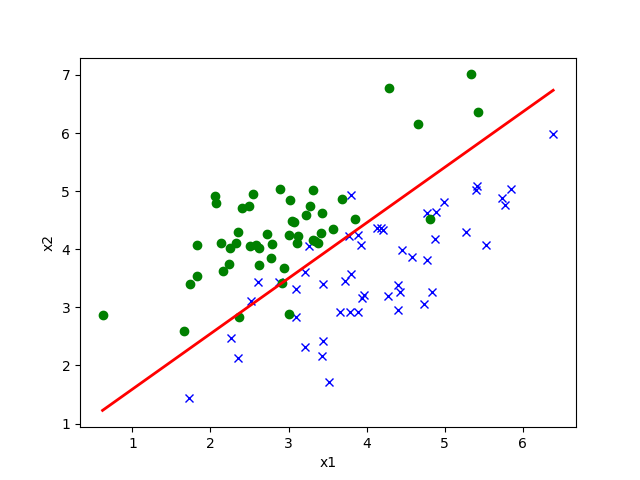
\includegraphics[width=0.6\textwidth]{p01e_pred_2_txt_gda_valid}
        \caption{GDA on Dataset 2}
    \end{figure}

 On Dataset 1 GDA seem to perform worse than Logistic Regression, this 
 is because dataset 1 doesn't look like Gaussian.
\end{answer}

}\fi

	\clearpage
\item \points{3 extra credit} For the dataset where GDA performed worse in
parts (f) and (g), can you find a transformation of the $x^{(i)}$'s such
that GDA performs significantly better? What is this transformation?

\ifnum\solutions=1{
  \begin{answer}

Observe the plot of dataset 1, on x1 axis the data point
on roughly follows Gaussian, but on x2 axis the point density 
looks like a exponential distribution which has a big head
and small a tail. It can also be seen as $\chi^2$ distribution,
which can be seen as sum of k Gaussians,  which leads to the 
first two transformation. 

The third log transformation also looking good.

    \begin{figure}[h]
        \centering
        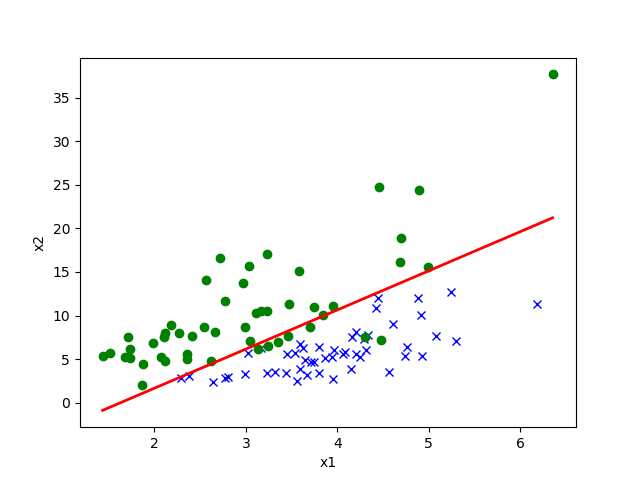
\includegraphics[width=0.6\textwidth]{p01e_pred_1_txt_gda_valid_2}
        \caption{ x2 = sqrt(x2) on validation set}
    \end{figure}
    
    \begin{figure}[h]
        \centering
        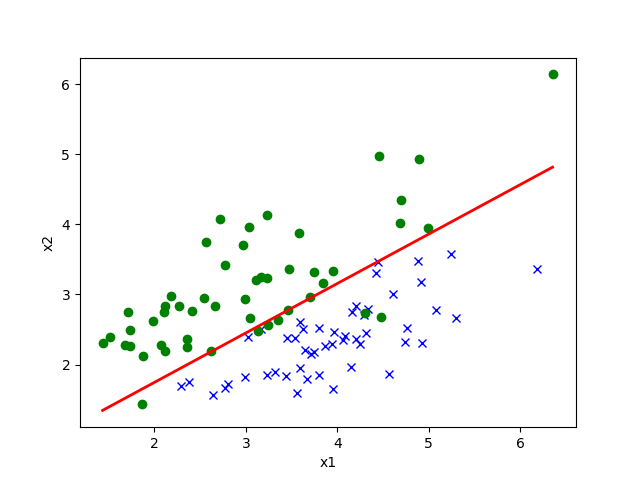
\includegraphics[width=0.6\textwidth]{p01e_pred_1_txt_gda_valid_4}
        \caption{ x2 = $(x2)^{\frac{1}{4}}$ on validation set }
    \end{figure}
    
    \begin{figure}[h]
        \centering
        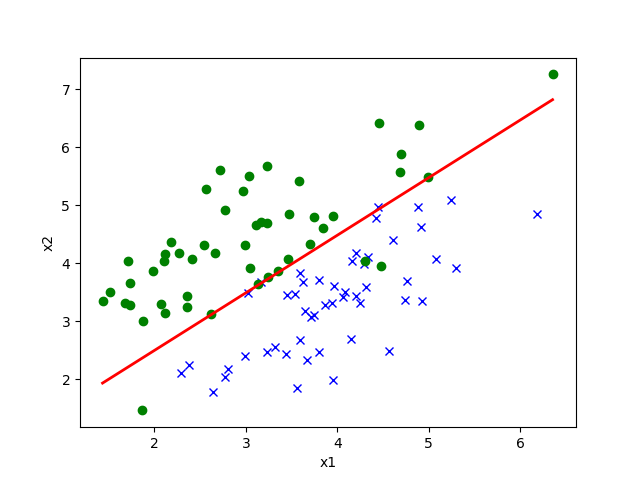
\includegraphics[width=0.6\textwidth]{p01e_pred_1_txt_gda_valid_log}
        \caption{ x2 = log(x2) validation set }
    \end{figure}

\end{answer}

}\fi

\end{enumerate}
